%
% CS 321: Homework 1
%
% Due date: October 9, 2013
%
\documentclass[12pt]{article}

\usepackage{amsmath}
\usepackage{amssymb}
\usepackage{amsthm}

\usepackage{geometry}

\usepackage{tikz}
\usetikzlibrary{arrows,automata}

\title{CS321 - Homework 2}
%\author{Trevor Bramwell}
\date{\today}

\begin{document}
\maketitle

%
% Section 2.2: 6, 7, 10a, 12, 14, 18
% Section 2.3: 6
%
\section*{Section 2.2}

% 6, 7, 10a, 12, 14, 18
\begin{description}
    \item[6] For the nfa in Figure 2.9, find $\delta^*(q_0, 1010)$ and $\delta^*(q_1, 00)$.

    \item[7] Design an NFA with no more than five states for the set

        $\{abab^n : n \ge 0\} \cup \{aba^n : n \ge 0\}$.

    \item[10(a)] Find an NFA with three states that accepts the language

        $L = \{a^n: n \ge 1\} \cup \{b^m a^k : m \ge 0, k \ge 0 \}$.

    \item[12] Which of the strings $00$, $01001$, $10010$, $000$, $0000$ are accepted by the following
        nfa?

        \begin{center}
        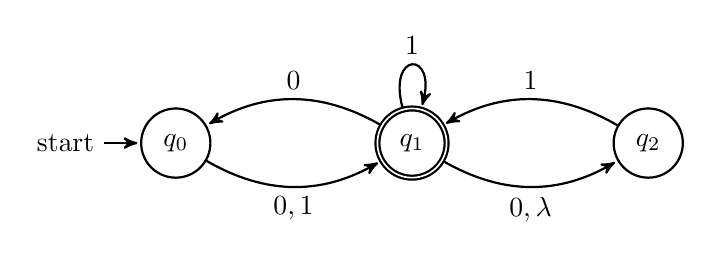
\begin{tikzpicture}[->,>=stealth',shorten >=1pt,auto,node distance=3cm,
                            thick]
          \tikzstyle{every state}=[fill=white]

          \node[state,initial]   (A)              {$q_0$};
          \node[state,accepting] (B) [right of=A] {$q_1$};
          \node[state]           (C) [right of=B] {$q_2$};

          \path (A) edge [bend right] node [below] {$0,1$} (B)
                (B) edge [bend right] node [below] {$0, \lambda$} (C)
                    edge [loop above] node {$1$} (B)
                    edge [bend right] node [above] {$0$} (A)
                (C) edge [bend right] node [above] {$1$} (B);
                
        \end{tikzpicture}
        \end{center}

 
    \item[14] Let $L$ be the language accepted by the nfa in Figure 2.8. Find an nfa that
        accepts $L \cup \{a^5\}$.


    \item[18] Consider the following modification of Definition 2.6. An nfa
        with multiple initial states is defined by the quintuple
        \begin{align*}
            M = (Q, \Sigma, \delta, Q_0, F),
        \end{align*}
        where $Q_0 \subseteq Q$ is a set of possible initial states. The
        language accepted by such an automaton is defined as
        \begin{align*}
            L(M) = \{w: \delta^*(q_O,w)\, \mathrm{contains},\, q_f,\,
                     \mathrm{for\, any}\; q_0 \in Q_0, q_f \in F\}.
        \end{align*}

        Show that for every ufa with multiple initial states there exists an
        nfa with a single initial state that accepts the same language.
\end{description}

\section*{Section 2.3}
\begin{description}
    \item[6] Is it true that for every nfa $M = (Q, \Sigma, \delta, q_o, F)$ the complement of $L(M)$ is
        equal to the set $\{w \in \Sigma^*, \delta^*(q_0, w) \cap (Q - F) \ne 0\}$? If so, prove it; if not,
        give a counterexample.
\end{description}

\end{document}
